\documentclass[tikz, border=1mm]{standalone}

\newcommand{\arst}{0.5}

\begin{document}
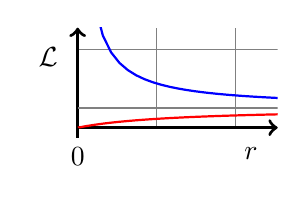
\begin{tikzpicture}[x=1in, y=1in, inner sep=0in, outer sep=0in, domain=0.001:1]

  \clip (-0.25, -0.25) rectangle (1, 0.5);

  \draw[very thin,color=gray] (0,0) grid (1,.5);

  \draw[->, very thick] (0,0) -- (0,0.5) node[anchor=north east, outer sep=0.1in] {$\mathcal{L}$};
  \draw[->, very thick] (0,0) -- (1,0) node[anchor=north east, outer sep=0.1in] {$r$};

  \draw[thick, gray]    plot (\x,{0.1});% node[anchor=west, outer sep=0.1in]{stable};
  \draw[thick, red]    plot (\x,{(10 * \x) * 0.1/(abs(10 * \x) + 5)});% node[anchor=north west, outer sep=0.1in]{contracts};
  \draw[thick, blue]    plot (\x,{0.1 * (10 * \x + 5)/(10 * \x + 0.1)});% node[anchor=south west, outer sep=0.1in]{expands};

  \draw[very thick, black] (0, 0) -- (0, -0.05) node[anchor=north, outer sep=0.05in] {$0$};

\end{tikzpicture}
\end{document}
